\chapter{Evaluation} \label{chapter:evaluation}

Evaluation must be conducted throughout the project to assess both the technical quantitative aspects of the project so that the project functions correctly and the qualitative aspects, such as the design and ease of use of the produced application.

Additional evaluation is then performed near the completion of the project in order to assess how well the project's objectives were achieved and whether the project can be considered a success.

%The evaluation can be split into two main categories:
%
%\begin{itemize}
%  \item \textbf{Quantitative evaluation:} assessing how well 
%\end{itemize}

\section{Software Validation}

Throughout the project, I ensured that each feature of the application was well tested to minimise bugs that could arise later on in the project. When implementing a feature in the project, the back-end element was normally completed and tested first to guarantee that when the front-end implementation was taking place I would be working with a fully-working element from the back-end. Testing was performed using the continuous integration tool Travis CI chosen in Section \ref{subsection:version-control}. This meant that tests were run automatically when commits were made to Git, allowing me to see at exactly what point any tests failed.

\subsection{API Testing}

The purpose of API testing is to ensure that all endpoints function correctly and handle any erroneous input as expected. Mocha **ref*** was the main testing framework used to test the API. It supports asynchronous callbacks, which is necessary for making calls to the API in test cases. Each test case is identified by a unique string to differentiate between each case and recognise which test cases have failed.

To make the actual API requests in a test case, the Supertest ***ref*** framework, allowing for assertions of HTTP requests. The structure of one of the test cases can be seen in Listing \ref{listing:api-test}. The \verb|describe()| and \verb|it()| functions specify the structure of the tests and uniquely identify each test case respectively, with the latter providing a \verb|done| function (line 3) to be called once the test case has finished executing its request. The HTTP request is made on line 4, where \verb|request| is a reference to the Supertest dependency, specifying the HTTP method and path (line 5). Subsequent functions are then called on this request to make assertions on elements of the response using the \verb|expect()| function (lines 6-11). In the example shown, these assertions include checking the response is of JSON type, checking that the HTTP response code is \textbf{200 OK} and checking the number of users returned is zero (since this particular request searches for a user with an invalid

\medskip

\begin{listing}
  \centering
  \begin{lstlisting}[language=javascript]
describe('GET /search/:userInfo', function() {
  describe('Valid user search', function () {
    it("should return empty array with name not found", function(done) {
      request(app)
        .get(uriPrefix + '/search/invalid name')
        .expect('Content-Type', /json/)
        .expect(function(res) {
          res.body.success.should.be.equal(true);
          res.body.users.should.have.length(0);
        })
        .expect(200, done);
    });
  });
});
  \end{lstlisting}
  \caption{Structure of a test case for the API}
  \label{listing:api-test}
\end{listing}

%The file that these test cases are written in is recognised by the project package to be the main test file for the project, meaning this test file is executed when the  \verb|test| command is run.  

The file that these test cases are written in is listed in the project's configuration file, so that this test file is automatically executed when the default \verb|test| command is run. When commits are made to Git, Travis CI then automatically runs the the \verb|test| command, indicating which test cases passed. If a test case failed, I was able to pinpoint the exact part of the endpoint that was affected due to the the unique names I gave to each test case. This was invaluable in speeding up the error fixing process.

\subsection{Mobile App Testing}

Testing the front-end mobile app was not performed in as much detail as the back-end, mainly because of forgetfulness and concentration on the implementation at hand. With that being said, many parts of the logic and UI of the application were tested thoroughly. To create a behaviour-driven development testing environment and provide English-like assertions by using the Quick ***ref*** and Nimble ***ref*** frameworks respectively, so as to match the way in which the API was tested.

Calls to the API were tested to ensure that responses were handled properly in \verb|APIManager|. In order to prevent unwanted requests to the API during testing, some HTTP requests were stubbed using the Mockingjay framework ***ref*** and mocked responses were returned to the app instead. For example, when making a valid request to register a new user, the actual API request is not made to prevent a superfluous record from being created in the database. In this case, a mocked response is returned containing a \textbf{200 OK} status code and the emulated successful response that would have been returned from the server. For invalid requests, no database records are ever created and so HTTP requests do not need to be mocked -- instead the actual error response returned from the API can be used in a test case.

To make sure that different components within the app worked together correctly, integration tests (or UI tests as they are known in iOS) were written. UI tests execute a sequence of operations within a simulator and use assertions to make sure each operation executes correctly.

% write more about integration tests

% talk about location simulation (gpx)

Thorough testing of the walk tracking feature was conducted to make sure that walk routes were accurate and points of interest were correctly displayed on the map. While testing by actually walking in the real world was extremely important, I was not restricted to this. Xcode provides a feature to simulate your location while running the app, either in the iOS simulator or on a real device. There are a number of default routes defined in Xcode to simulate a location route around California, however these were not so useful as not many points of interest were found there.

You can also define your own routes to use if you wish. The routes are stored as a list of coordinates in a GPX file that Xcode can then parse. I discovered a website ***ref*** that converts a route from Google Maps into a GPX file. I was able to use this tool to create routes in London where there are a large number of plaques, which was extremely useful for testing.

\section{User Testing}

I aimed to provide users with versions of the application as early as possible and often throughout the project so as to gain feedback frequently and iterate the application multiple times throughout the project based on this feedback. The feedback that was received from users ranged from bug fixes in the application to subjective views on features of the app that could be improved or changed.

\subsection{Bug Fixes}

The following section lists some of the bugs that were found in my code based on feedback from testing my application in the real world, either by myself or from other users that I provided the app to. For each error that was found, the reason that this error occurred and the solution that fixed the error is also listed.

\noindent \textbf{Error:} app crashes making any network request with no internet connection.

\begin{itemize}
  \item \textbf{Reason:} every time a network request is made in \verb|APIManager|, the status code of the response is obtained to see if an error has been returned. However, if there is no internet connection, there is no response from the request and so the status code is empty. This results in the Swift equivalent of a null pointer error, causing the app to crash.
  
  \item \textbf{Solution:} the status code of the response is only used if the response itself is not null, otherwise a default network error is returned.
\end{itemize}
  
\noindent \textbf{Error:} app crashes when creating an account after scrolling the text fields off screen.

\begin{itemize}
  \item \textbf{Reason:} table view cells in iOS are reusable, meaning the cells and their associated data that are not on the screen are not in memory and are recreated when they reappear on the screen. When pressing the button to create an account, the data the user entered from the text fields in the table view cells is retrieved and passed to the \verb|register()| function in \verb|APIManager|. If one or more of the cells is not on the screen, its data does not exist due to its reusability and so a null pointer error occurs when trying to obtain the value passed into \verb|register()|.
  
  \item \textbf{Solution:} instead of retrieving the data from cells when pressing the register button, a global class array was used to store the data from the cells as the user is entering it. This means that even if some cells are not on the screen when registering, the data is still stored previously and can be passed to the \verb|register()| function without any danger of any parameters being null.
\end{itemize}
  
\noindent \textbf{Error:} when tracking a particularly long walk, the image produced contains rendering issues where the map route is blurred, as shown in Figure \ref{fig:map-render-bug}.

\begin{figure}[hbt]
  \centering
  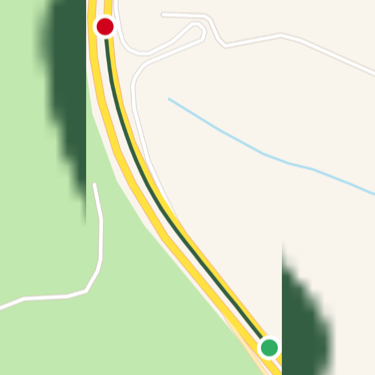
\includegraphics[width=0.5\textwidth]{map-render-bug}
  \caption{A bug in the app causing a walk's route to not render properly.}
  \label{fig:map-render-bug}
\end{figure}


\begin{itemize}
  \item \textbf{Reason:} the walk route image was produced by rendering an image of the visible map view on the screen using Core Graphics -- a framework used in iOS to perform 2D drawing. To do this, the map view needs to be zoomed out so that the entire walk route is fit in the view. In doing so, the polyline used to draw the walk route on the map, discussed in Section \ref{section:tracking-walks}, did not always render properly for reasons that I was not able to discover.
  
  \item \textbf{Solution:} the \verb|MKMapSnapShotter| class, part of the MapKit framework, was used to render an image of a map rather than using Core Graphics. By specifying a coordinate region and various other options, an image is rendered of that area of a map. The map route still had to be rendered separately onto the map afterwards using Core Graphics, but I found this was the best solution at the time to avoid the rendering issues presented by the previous method.
\end{itemize}

\subsection{Final Survey}

% make qualitative evaluation into quantitive
% survey on ease of use, design, rating of features, etc.

When the implementation phase of the project was completed, I conducted a survey about the app as a way to try and quantify the qualitative aspects of the project that needed to be evaluated. These qualitative aspects include the ease of use of the application, its design and how useful each feature is to the user. The full results of this survey can be seen in Appendix \ref{appendix:final-survey}, with a summary of results discussed below. Any question where the user was expected to rate a feature's usefulness a linear scale from 1 to 5 was given to choose from, with 5 being the most useful and 1 not useful at all.

The survey showed that both design and ease of use of the application appealed to the user, with no responses for either category giving a score less than 3. The main questions asking the user whether they were encouraged to walk more when using the app gave mainly positive results, with 73\% of people giving a score of 3 or 4. The rating of features gave mixed responses, with the controversial features being tracking walks and walk invitations. Features to view points of interest and view walks on your profile provided the best responses in the survey, with all users giving a score of at least 3.

An interesting point to discuss is the opinion of users who had used previous walking or fitness apps compared to those who hadn't. From the graph in Figure \ref{fig:survey-graph}, we can see that the users who have used previous fitness applications gave lower scores for the tracking walks and statistics features of my app. This is understandable since the apps that these users have used, the most popular being Strava and Runkeeper, are dedicated fitness and running apps whereas the tracking of walks in my application is only one element.

\begin{figure}[htb]
    \centering
    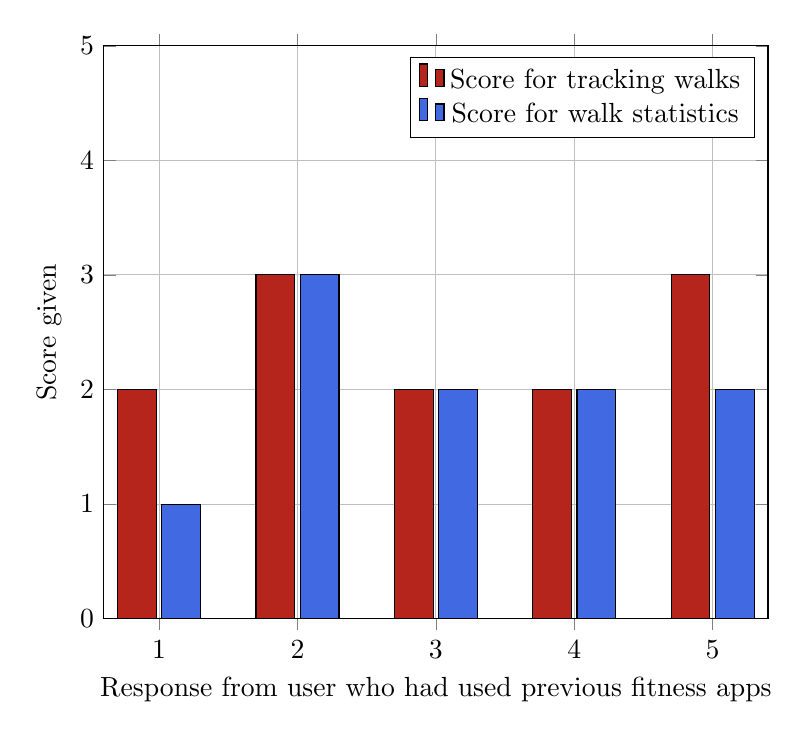
\begin{tikzpicture}
    \begin{axis}[xlabel=Response from user who had used previous fitness apps,
                ylabel=Score given,
                scale only axis,
                % enlargelimits=false,
                ymin=0,
                ymax=5,
                ybar,
                grid=both,
                % minor tick num=5,
                bar width=14pt,
                clip mode=individual]
        \addplot[fill=BrickRed] coordinates{
        (1,2)
        (2,3)
        (3,2)
        (4,2)
        (5,3)
        };
        
        \addplot[fill=RoyalBlue] coordinates{
        (1,1)
        (2,3)
        (3,2)
        (4,2)
        (5,2)
        };
        
        \legend{Score for tracking walks, Score for walk statistics}
    \end{axis}
    \end{tikzpicture}
    \caption{Graph showing the scores for the feature ratings of tracking walks and viewing walk statistics, given by users who had previously used walking or fitness apps}
    \label{fig:survey-graph}
\end{figure}

Additional comments were left by users at the end of the survey. The main points written were that other fitness apps that users have used were better for fitness and provided more detailed statistics, and other points of interest should be used instead of just historical plaques. I also conducted hallway testing, where I asked strangers to give their opinion on my application having no prior knowledge of it. The results from hallway testing agreed mainly agreed with the results of the survey, with people liking the design of the app and the main concept, but some stating that some other points of interest should be used and more achievements added.

I concluded from this survey that I have created an application that has a sleek design and is very easy to use, with multiple features that users found useful. Having said this, I also found that there were a few limitations in some features in the app that need to be addressed in order to make it cater for a wider audience.

\section{Objective Reflection}

% gauge if project is success

One way to gauge whether the project can be considered a success is to reflect back on the broad objectives proposed in Section \ref{section:objectives}. The objectives are listed below, each with an explanation as to whether it was achieved as a result of the quantitative and qualitative evaluation discussed in the previous two sections.

\begin{enumerate}[label=\textbf{Obj \arabic*}]
  \item \textbf{Encourage walking:} the basic features aimed to achieve this objective, namely inviting users to go on a walk and gamification, were implemented. User testing yielded that the tracking walks feature was maybe not up to scratch compared to existing fitness applications, which is understandable. The gamification aspect was popular, but more achievements need to be added in order to encourage the user to walk more. Based on this, I can conclude that although the basic features were implemented, this objective was not fully achieved.

  \item \textbf{Help discover the world:} the points of interest feature was implemented as I had planned and so I would say this objective was mainly achieved. The survey results showed that the plaques displayed on the map when tracking a walk was one of the most popular features in the app. A few users were not satisfied with just plaques being shown and would like other points of interest to be used, which is something that would be implemented in the future.

  \item \textbf{Test and evaluate with real users:} throughout the project the app was given to known and unknown users to test and evaluate the app. From the final survey, the majority of users have stated that the app encouraged them to walk and exercise more. Based on this, I can constitute this objective as a success.
\end{enumerate}

\subsection{Project Management}

To reflect on how well I managed my time during the project I compared the original project plan proposed at the start of the project to the actual time taken to complete each task. The comparison between the two can be seen in Table \ref{table:project-timeline-comparison}.

I had planned to implement a great deal of the project, including setting up the back-end and skeleton app, before the exams at the end of the second term on \nth{20} March so as to provide myself with a platform to continue the project after this date. In reality however, due to the combination of the workload I had during this time and the steep learning curve for implementing the back-end, I did not implement as much as I had hoped.

Furthermore, I did not anticipate how long the initial phase of the API implementation would take me. I had no experience in Javascript or any back-end development before the start of the project and so there was a much steeper learning curve to that of the front-end development.

% talk about API tutorials



On the other hand, some of the front-end features actually took a shorter amount of time than what I had planned. For example, inviting users to go on a walk actually only took around two weeks to implement rather than the three weeks I had outlined in Table \ref{table:project-timeline-comparison}, meaning that I gained some time back from the time lost implementing the API setup.

I had made sure to allow for extra time at the end of the implementation phase so that the problems listed above did not hinder the project and I was able to complete my intended features in time, albeit not having enough time to implement the extensions I had planned before the project. These were formulated into future extensions, which are listed in detail in Section \ref{section:future-work}.

\begin{table}[hbt]
  \centering
  \begin{tabular}{|l|| *{16}{c|}}
    \hline
    \multicolumn{17}{|c|}{\textsc{Proposed}}\\
    \hline
    \multirow{2}{*}{\textbf{Activity}} & \multicolumn{3}{c|}{\textbf{February}} & \multicolumn{4}{c|}{\textbf{March}} & \multicolumn{4}{c|}{\textbf{April}} & \multicolumn{5}{c|}{\textbf{May}}\\
    \cline{2-17}
    & 13 & 20 & 27 & 6 & 13 & 20 & 27 & 3 & 10 & 17 & 24 & 1 & 8 & 15 & 22 & 29\\
    \hline
    Skeleton app & \cellcolor{BrickRed} &&&& \multirow{9}{*}{\rotatebox[origin=c]{90}{\textls{REVISION}}} & \multirow{9}{*}{\rotatebox[origin=c]{90}{\textls{EXAMS}}} &&&&&&&&&&\\
    \hhline{*{5}{-}~~*{10}{-}}
    Set up web server &\multicolumn{2}{c|}{\cellcolor{BrickRed}}&&&&&&&&&&&&&&\\
    \hhline{*{5}{-}~~*{10}{-}}
    Set up database &\multicolumn{2}{c|}{\cellcolor{BrickRed}}&&&&&&&&&&&&&&\\
    \hhline{*{5}{-}~~*{10}{-}}
    Login system &&& \multicolumn{2}{c|}{\cellcolor{BrickRed}}&&&&&&&&&&&&\\
    \hhline{*{5}{-}~~*{10}{-}}
    Track walks &&&& \cellcolor{BrickRed} &&& \cellcolor{BrickRed} &&&&&&&&&\\
    \hhline{*{5}{-}~~*{10}{-}}
    User profile &&&&&&&& \multicolumn{2}{c|}{\cellcolor{BrickRed}}&&&&&&&\\
    \hhline{*{5}{-}~~*{10}{-}}
    Invite users for walk &&&&&&&&&&\multicolumn{3}{c|}{\cellcolor{BrickRed}}&&&&\\
    \hhline{*{5}{-}~~*{10}{-}}
    Gamification &&&&&&&&&&&&&\multicolumn{2}{c|}{\cellcolor{BrickRed}}&&\\
    \hhline{*{5}{-}~~*{10}{-}}
    Extensions &&&&&&&&&&&&&&&\multicolumn{2}{c|}{\cellcolor{BrickRed}}\\
    \hline
    \hline
    \multicolumn{17}{|c|}{\textsc{Actual}}\\
    \hline
    \multirow{2}{*}{\textbf{Activity}} & \multicolumn{3}{c|}{\textbf{February}} & \multicolumn{4}{c|}{\textbf{March}} & \multicolumn{4}{c|}{\textbf{April}} & \multicolumn{5}{c|}{\textbf{May}}\\
    \cline{2-17}
    & 13 & 20 & 27 & 6 & 13 & 20 & 27 & 3 & 10 & 17 & 24 & 1 & 8 & 15 & 22 & 29\\
    \hline
    Skeleton app && \multicolumn{2}{c|}{\cellcolor{OliveGreen}} && \multirow{10}{*}{\rotatebox[origin=c]{90}{\textls{REVISION}}} & \multirow{10}{*}{\rotatebox[origin=c]{90}{\textls{EXAMS}}} &&&&&&&&&&\\
    \hhline{*{5}{-}~~*{10}{-}}
    Set up web server &&&& \cellcolor{OliveGreen} &&& \cellcolor{OliveGreen} &&&&&&&&&\\
    \hhline{*{5}{-}~~*{10}{-}}
    Set up database &&&& \cellcolor{OliveGreen} &&& \cellcolor{OliveGreen} &&&&&&&&&\\
    \hhline{*{5}{-}~~*{10}{-}}
    Login system &&&&&&& \multicolumn{2}{c|}{\cellcolor{OliveGreen}}&&&&&&&&\\
    \hhline{*{5}{-}~~*{10}{-}}
    Track walks &&&&&&&&& \multicolumn{3}{c|}{\cellcolor{OliveGreen}}&&&&&\\
    \hhline{*{5}{-}~~*{10}{-}}
    User profile &&&&&&&&&&&&\multicolumn{2}{c|}{\cellcolor{OliveGreen}}&&&\\
    \hhline{*{5}{-}~~*{10}{-}}
    Invite users for walk &&&&&&&&&&&&&&&\multicolumn{2}{c|}{\cellcolor{OliveGreen}}\\
    \hhline{*{5}{-}~~*{10}{-}}
    Gamification &&&&&&&&&&&&&&\cellcolor{OliveGreen}&&\\
    \hhline{*{5}{-}~~*{10}{-}}
    Extensions &&&&&&&&&&&&&&&&\\
    \hline
  \end{tabular}
  \caption{Comparison between the proposed schedule for the project (top) and the actual schedule (bottom).}
  \label{table:project-timeline-comparison}
\end{table}

\section{Summary}

Based on the evaluation conducted in this chapter, I believe I have created a fully functioning and well tested application that achieved most of my initial objectives. The final application does however have many limitations that were noticed by both myself and other users during testing. 

We have found that the RESTful style of the API provided an elegant way to interact with the database. The categorised structure that was defined meant that each endpoint in the API had a single functionality to read from or write to the database, and once the base structure was implemented it was very easy to add or remove endpoints.

We have also found that JSON used in HTTP requests to communicate between the mobile app and the API worked well, owing to the flexibility and structure of the notation. JSON could be parsed and constructed by both the front and back-end, allowing for easy data transfer.

